\documentclass[a4paper]{report}
% Some basic packages
\usepackage[utf8]{inputenc}
\usepackage[T1]{fontenc}
\usepackage{textcomp}
\usepackage[english]{babel}
\usepackage{url}
\usepackage{graphicx}
\usepackage{float}
\usepackage{booktabs}
\usepackage{enumitem}

\pdfminorversion=7

% Don't indent paragraphs, leave some space between them
\usepackage{parskip}

% Hide page number when page is empty
\usepackage{emptypage}
\usepackage{subcaption}
\usepackage{multicol}
\usepackage{xcolor}

% Other font I sometimes use.
% \usepackage{cmbright}

% Math stuff
\usepackage{amsmath, amsfonts, mathtools, amsthm, amssymb}
% Fancy script capitals
\usepackage{mathrsfs}
\usepackage{cancel}
% Bold math
\usepackage{bm}
% Some shortcuts
\newcommand\N{\ensuremath{\mathbb{N}}}
\newcommand\R{\ensuremath{\mathbb{R}}}
\newcommand\Z{\ensuremath{\mathbb{Z}}}
\renewcommand\O{\ensuremath{\emptyset}}
\newcommand\Q{\ensuremath{\mathbb{Q}}}
\newcommand\C{\ensuremath{\mathbb{C}}}
\renewcommand\L{\ensuremath{\mathcal{L}}}

% Package for Petri Net drawing
\usepackage[version=0.96]{pgf}
\usepackage{tikz}
\usetikzlibrary{arrows,shapes,automata,petri}
\usepackage{tikzit}
\input{petri_nets_style.tikzstyles}

% Easily typeset systems of equations (French package)
\usepackage{systeme}

% Put x \to \infty below \lim
\let\svlim\lim\def\lim{\svlim\limits}

%Make implies and impliedby shorter
\let\implies\Rightarrow
\let\impliedby\Leftarrow
\let\iff\Leftrightarrow
\let\epsilon\varepsilon

% Add \contra symbol to denote contradiction
\usepackage{stmaryrd} % for \lightning
\newcommand\contra{\scalebox{1.5}{$\lightning$}}

% \let\phi\varphi

% Command for short corrections
% Usage: 1+1=\correct{3}{2}

\definecolor{correct}{HTML}{009900}
\newcommand\correct[2]{\ensuremath{\:}{\color{red}{#1}}\ensuremath{\to }{\color{correct}{#2}}\ensuremath{\:}}
\newcommand\green[1]{{\color{correct}{#1}}}

% horizontal rule
\newcommand\hr{
    \noindent\rule[0.5ex]{\linewidth}{0.5pt}
}

% hide parts
\newcommand\hide[1]{}

% si unitx
\usepackage{siunitx}
\sisetup{locale = FR}

% Environments
\makeatother
% For box around Definition, Theorem, \ldots
\usepackage{mdframed}
\mdfsetup{skipabove=1em,skipbelow=0em}
\theoremstyle{definition}
\newmdtheoremenv[nobreak=true]{definitie}{Definitie}
\newmdtheoremenv[nobreak=true]{eigenschap}{Eigenschap}
\newmdtheoremenv[nobreak=true]{gevolg}{Gevolg}
\newmdtheoremenv[nobreak=true]{lemma}{Lemma}
\newmdtheoremenv[nobreak=true]{propositie}{Propositie}
\newmdtheoremenv[nobreak=true]{stelling}{Stelling}
\newmdtheoremenv[nobreak=true]{wet}{Wet}
\newmdtheoremenv[nobreak=true]{postulaat}{Postulaat}
\newmdtheoremenv{conclusie}{Conclusie}
\newmdtheoremenv{toemaatje}{Toemaatje}
\newmdtheoremenv{vermoeden}{Vermoeden}
\newtheorem*{herhaling}{Herhaling}
\newtheorem*{intermezzo}{Intermezzo}
\newtheorem*{notatie}{Notatie}
\newtheorem*{observatie}{Observatie}
\newtheorem*{exe}{Exercise}
\newtheorem*{opmerking}{Opmerking}
\newtheorem*{praktisch}{Praktisch}
\newtheorem*{probleem}{Probleem}
\newtheorem*{terminologie}{Terminologie}
\newtheorem*{toepassing}{Toepassing}
\newtheorem*{uovt}{UOVT}
\newtheorem*{vb}{Voorbeeld}
\newtheorem*{vraag}{Vraag}

\newmdtheoremenv[nobreak=true]{definition}{Definition}
\newtheorem*{eg}{Example}
\newtheorem*{notation}{Notation}
\newtheorem*{previouslyseen}{As previously seen}
\newtheorem*{remark}{Remark}
\newtheorem*{note}{Note}
\newtheorem*{problem}{Problem}
\newtheorem*{observe}{Observe}
\newtheorem*{property}{Property}
\newtheorem*{intuition}{Intuition}
\newmdtheoremenv[nobreak=true]{prop}{Proposition}
\newmdtheoremenv[nobreak=true]{theorem}{Theorem}
\newmdtheoremenv[nobreak=true]{corollary}{Corollary}

% End example and intermezzo environments with a small diamond (just like proof
% environments end with a small square)
\usepackage{etoolbox}
\AtEndEnvironment{vb}{\null\hfill$\diamond$}%
\AtEndEnvironment{intermezzo}{\null\hfill$\diamond$}%
% \AtEndEnvironment{opmerking}{\null\hfill$\diamond$}%

% Fix some spacing
% http://tex.stackexchange.com/questions/22119/how-can-i-change-the-spacing-before-theorems-with-amsthm
\makeatletter
\def\thm@space@setup{%
  \thm@preskip=\parskip \thm@postskip=0pt
}


% Exercise 
% Usage:
% \exercise{5}
% \subexercise{1}
% \subexercise{2}
% \subexercise{3}
% gives
% Exercise 5
%   Exercise 5.1
%   Exercise 5.2
%   Exercise 5.3
\newcommand{\exercise}[1]{%
    \def\@exercise{#1}%
    \subsection*{Exercise #1}
}

\newcommand{\subexercise}[1]{%
    \subsubsection*{Exercise \@exercise.#1}
}


% \lecture starts a new lecture (les in dutch)
%
% Usage:
% \lecture{1}{di 12 feb 2019 16:00}{Inleiding}
%
% This adds a section heading with the number / title of the lecture and a
% margin paragraph with the date.

% I use \dateparts here to hide the year (2019). This way, I can easily parse
% the date of each lecture unambiguously while still having a human-friendly
% short format printed to the pdf.

\usepackage{xifthen}
\def\testdateparts#1{\dateparts#1\relax}
\def\dateparts#1 #2 #3 #4 #5\relax{
    \marginpar{\small\textsf{\mbox{#1 #2 #3 #5}}}
}

\def\@lecture{}%
\newcommand{\lecture}[3]{
    \ifthenelse{\isempty{#3}}{%
        \def\@lecture{Lecture #1}%
    }{%
        \def\@lecture{Lecture #1: #3}%
    }%
    \subsection*{\@lecture}
    \marginpar{\small\textsf{\mbox{#2}}}
}



% These are the fancy headers
\usepackage{fancyhdr}
\pagestyle{fancy}

% LE: left even
% RO: right odd
% CE, CO: center even, center odd
% My name for when I print my lecture notes to use for an open book exam.
% \fancyhead[LE,RO]{Gilles Castel}

\fancyhead[RO,LE]{\@lecture} % Right odd,  Left even
\fancyhead[RE,LO]{}          % Right even, Left odd

\fancyfoot[RO,LE]{\thepage}  % Right odd,  Left even
\fancyfoot[RE,LO]{}          % Right even, Left odd
\fancyfoot[C]{\leftmark}     % Center

\makeatother




% Todonotes and inline notes in fancy boxes
\usepackage{todonotes}
\usepackage{tcolorbox}

% Make boxes breakable
\tcbuselibrary{breakable}

% Verbetering is correction in Dutch
% Usage: 
% \begin{verbetering}
%     Lorem ipsum dolor sit amet, consetetur sadipscing elitr, sed diam nonumy eirmod
%     tempor invidunt ut labore et dolore magna aliquyam erat, sed diam voluptua. At
%     vero eos et accusam et justo duo dolores et ea rebum. Stet clita kasd gubergren,
%     no sea takimata sanctus est Lorem ipsum dolor sit amet.
% \end{verbetering}
\newenvironment{verbetering}{\begin{tcolorbox}[
    arc=0mm,
    colback=white,
    colframe=green!60!black,
    title=Opmerking,
    fonttitle=\sffamily,
    breakable
]}{\end{tcolorbox}}

% Noot is note in Dutch. Same as 'verbetering' but color of box is different
\newenvironment{noot}[1]{\begin{tcolorbox}[
    arc=0mm,
    colback=white,
    colframe=white!60!black,
    title=#1,
    fonttitle=\sffamily,
    breakable
]}{\end{tcolorbox}}




% Figure support as explained in my blog post.
\usepackage{import}
\usepackage{xifthen}
\usepackage{pdfpages}
\usepackage{transparent}
\newcommand{\incfig}[1]{%
    \def\svgwidth{\columnwidth}
    \import{./figures/}{#1.pdf_tex}
}

% Fix some stuff
% %http://tex.stackexchange.com/questions/76273/multiple-pdfs-with-page-group-included-in-a-single-page-warning
\pdfsuppresswarningpagegroup=1


% My name
\author{Bruno M. Pacheco}

 
\begin{document}
 
\title{Lista 1}
\author{Bruno M. Pacheco (16100865)\\
DAS5151 - Instrumentação em Controle}
 
\maketitle
 
\exercise{1}

No momento da alta do sinal, com $V_{in} = 10\,V$, temos, assumindo uma queda de $0,7\,V$ na junção BE do transistor, uma corrente $I_B = \frac{10}{245520} = 40,72\,\mu A$, o que resultaria em uma corrente $I_C = \beta I_B = 4,89\,mA$. Para isso, precisaríamos de uma queda de tensão de mais de 10 V sobre o resistor no coletor do transistor, ou uma queda de tensão negativa na junção CE do transistor. Isso nos indica que o transistor está atuando já na zona de saturação no período de alta do sinal de entrada.

Assumindo 1,0 V de queda na junção CE do transistor no período de condução (saturação), teremos um sinal de saída como na figura abaixo.

\begin{figure}[H]
    \centering
    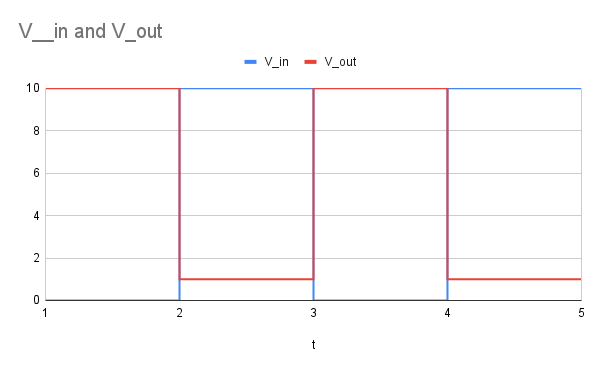
\includegraphics[width=0.8\textwidth]{figures/lista1-1.png}
\end{figure}

\exercise{2}

Pela construção do circuito, espera-se uma corrente fluindo pelo diodo $I_Z = \frac{V_S - 15}{R_S}$. Pela especificação de potência do diodo, sabemos que a corrente máxima que ele suporta é \[
I_{Z,max} = \frac{0,5}{15} = 33,33\,mA
.\] Dessa forma, \[
    \frac{V_S - 15}{R_S} < I_{Z,max} \implies R_S > 750,76\,\Omega
.\] 

\exercise{3}

A impedância vista pela fonte é $Z=11500 + j6000$. Assim, podemos calcular a queda de tensão na impedância do multímetro \[
V_{out} = \frac{V_{in}}{Z} 10000 = \frac{V_{in}}{1,15 + j0,6} \implies \|V_{out}\| = 0,7709 \|V_{in}\|
.\] Ou seja, teremos um erro de 22,81\%.

\exercise{4}

Pelas especificações informadas, o motor precisa de $250\,mA$. Isso já elimina o BC547, uma vez é especificado para operar com no máximo $100\,mA$ de corrente de coletor.

Já o 2N4401 pode operar com até $600\,mA$ no coletor, além de possuir um ganho mínimo de 40 quando operando com corrente de coletor de $500\,mA$, o que indica que precisaríamos de $6,25\,mA$ de corrente de base vindo do Arduino, o que se encontra dentro dos seus limites de operação. Ou seja, mesmo acionando o motor de forma contínua estaríamos dentro dos limites do Arduino e do transistor caso fosse utilizado o 2N4401 e um resistor de base apropriado.

\exercise{5}

O circuito proposto para acionar uma carga $R_L$ é como abaixo, dado um condicionamento ideal dos resistores e transistores envolvidos.

\begin{figure}[H]
    \centering
    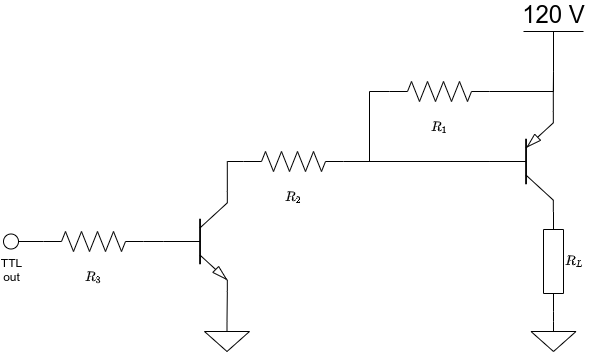
\includegraphics[width=0.8\textwidth]{figures/lista1-5.png}
\end{figure}

Caso fosse utilizado um resistor NPN entre a carga e a fonte, seria necessário um acionamento de alta tensão, o que não seria possível dadas as especificações da placa de aquisição de dados. Caso fosse utilizado um transistor NPN conectado entre a carga e o terminal comum do circuito, a junção CB do transistor seria o calcanhar de aquiles, uma vez que falhando poderia expor a placa de aquisição à alta tensão, além de manter a carga sempre conectada à alta tensão, ou seja, seria possível fechar o circuito da carga caso ela fosse conectada de alguma outra forma ao terminal comum.

\exercise{6}

\subexercise{a}

Definindo $R_i = 10\,M\Omega$ e $R_o = 75\,\Omega$ os resistores de entrada e de saída do LM741, analisamos o circuito como na figura abaixo.

\begin{figure}[H]
    \centering
    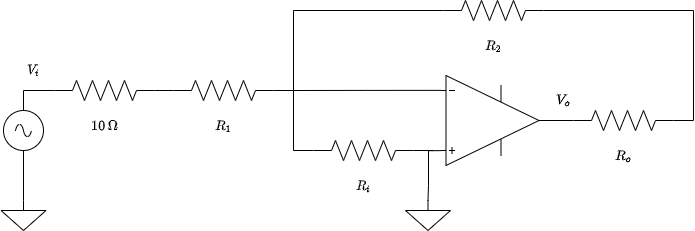
\includegraphics[width=0.8\textwidth]{figures/lista1-6a.png}
\end{figure}

Para simplificar a análise, definimos $R_1' = R_1 + 10\,\Omega$ e $R_2'=R_2+R_o$. Agora, analisando o nó de $V^{-}$, a tensão no terminal inversor do amplificador operacional, e resolvendo também as malhas que envolvem esse e $V_i$ e $V_o$, pode-se chegar na relação \[
V^{-} = \frac{R_i\left( R_1'V_i+R_2'V_o \right) }{1+R_i\left( R_1'+R_2' \right) }
.\] Também temos que $V_o = A\left( V^{+}-V^{-} \right) = -A V^{-}$, logo, pode-se chegar na relação \[
\frac{V_o}{V_i} = \frac{-AR_iR_2'}{1+R_i\left( R_1'+R_2' \right) +AR_iR_1'} \tag{$*$}
.\] 

Para a situação proposta, teremos $V_i = 1\,mV$ e $A_{3\,kHz} = 50 dB \approx 316,23$. Dessa forma, por $(*)$, encontra-se $V_o \approx 45,82\,mV$ de amplitude.

\subexercise{b}

Em um sistema ideal, \[
\lim_{A,R_i \to \infty} \frac{V_o}{V_i} = \frac{-R_2'}{R_1'}
.\] Considerando ainda que as impedâncias de saída e as impedâncias de entrada são todas nulas, teríamos o ganho de 100 esperado. Nesse caso, esperaríamos um sinal de saída $V_{o,ideal}=100\,mV$. Ou seja, um erro de 54,18\%.

\subexercise{c}

Mesmo considerando um amplificador ideal ($A,R_i \to \infty$), podemos melhorar a estimativa do ganho considerando as impedâncias de saída do transdutor e do amplificador operacional. Ou seja, aproximamos o ganho do circuito por \[
\frac{V_o}{V_i}' = \frac{R_2+R_o}{R_1+10} = 100
.\] Dessa forma, pode-se escolher $R_1=10\,\Omega$ e $R_2=1925\,\Omega$, o que resultaria, por $(*)$, em um ganho de \[
    \frac{V_o}{V_i} = 75,79
,\] ou seja, um erro de 24.21\%. Ainda melhores resultados podem ser obtidos a partir da iterações de valores em cima de $(*)$.

\exercise{7}

Pelas especificações, encontramos $\tau \approx 136,4\,ms$, o que nos permite modelar o sistema de transmissão como \[
    G(s) = \frac{1}{1+\tau s}
.\] Assim, queremos \[
\|G(j2\pi60)\| = \|\frac{1}{1+\tau\pi120}\| \approx 0,02
,\] ou seja, o sinal terá somente 2\% da sua amplitude original.

\exercise{8}

A partir dos dados do transdutor, podemos determinar $\tau=50$, o que nos da uma frequência de corte $f_c = 0,0032\,Hz$. Então, para encontrar a frequência na qual há 5\% de atenuação, resolvemos \[
\frac{1}{\sqrt{1+ \left( \frac{f_c}{f} \right) ^2} } = 0,95 \implies f = 0,0097\,Hz
.\] 

Como o sistema se comporta como um passa alta, teremos uma atenuação menor com uma frequência acima da encontrada.

\exercise{9}

Pela dissipação máxima de potência, encontramos $I_{max} = 33,33\,mA$, que é a corrente quando a queda de tensão sobre o LED é menor (ou seja, a queda de tensão sobre o resistor é maior). Além disso, nessa situação, a queda de tensão sobre o resistor é de 2 V, ou seja, \[
I = \frac{2}{R} < 0,03333 \implies R > 60\,\Omega
.\]

\exercise{10}

Para esse problema, será utilizado o circuito abaixo como referência já sendo substituído o amplificador operacional pelo seu circuito equivalente, onde $R_e = 10^9$.

\begin{figure}[H]
    \centering
    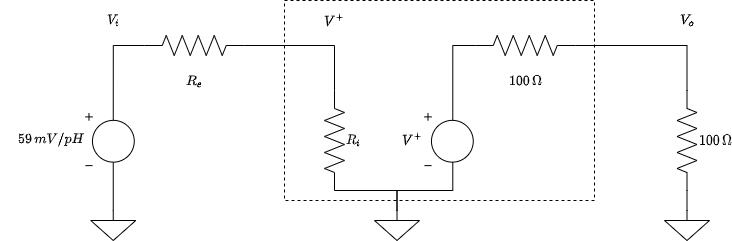
\includegraphics[width=0.8\textwidth]{figures/lista1-10.png}
\end{figure}

\subexercise{a}

Pelo circuito, é fácil ver que $V_o = \frac{V^+}{2}$. Dessa forma, precisamos que, para $pH=15$, $V^+=200\,mV$ para que seja utilizada toda a escala do registrador. Além disso, $pH=15\implies V_i = 885\,mV$ e \[
V^+ = R_i \frac{V_i}{R_e+R_i} \implies R_i = \frac{R_e V^+}{V_i - V^+} = 2,920.10^8
.\]

Já a sensibilidade do indicador deve ser tal que em $100\,mV$ ele indique 15 de pH, ou seja, sensibilidade de $0,15\,pH/mV$.

\subexercise{b}

Nesse caso, ter-se-ia, com $PH=7 \implies V_i = 413\,mV$, $V^+ = 52,61\,mV$. Isso resultaria em $V_o = 26,31\,mV$ e, portanto, com a sensibilidade proposta, uma indicação de pH de 3,95. Ou seja, um erro de -20,36\% em relação ao fundo de escala.

\end{document}
